\section{Class Structure and Scheduling}

Previously we broke down the requirements for the functionality of the bus into a number of components, and created a class diagram \todo{Can I call it a class diagram? Call it something else if I change it.} to structure how those would interact. The next step is to create interfaces and thereby clear, concrete contracts of the intended functionality of each major class in the program. 

In non real-time systems the class and system structure may be enough to start creating interfaces, but in this case we still need to figure out we will reconcile the class structure with the chosen scheduling method. As mentioned in \ref{analysis:scheduling}, we will be using fixed priority scheduling to decide when the tasks in the bus are run. 

One of the questions that we need to clear up is where we run the program from and where the main function resides. Where do we initialise our components and ensure that they deliver their data to the correct receiver? Besides answering these questions, we must ensure that conventions of good object-oriented design are still followed. Specifically, the trouble is keeping a low coupling between the components, even though they all need to communicate with the driving-component. 

\subsubsection{Program Flow}
The program flow and main function is defined within the .oil-files; see a description of these in section \ref{OILteo}. Inside the .oil-files we define functions as tasks which will be called with specific priorities, periods and deadlines. 

The ObstacleDetection-component (uses the ultrasonic sensor to check for obstacles ahead of the vehicle) will be used as an example to illustrate the issue. If the program did not have to be a real-time system, then the obvious solution would simply be to detect obstacles regularly. If any are found, then the Driving-component is immediately alerted, which then calls the motor controls and adjust the direction of the bus.

The issue in this case is that the bus might miss a lot of other deadlines while the Driving-component has control of the CPU. This is of course unacceptable, because, depending on the circumstances, the bus might no longer meet its other requirements. 

Imagine the following worst case. The bus detects a bus stop and decides to park there. Now the driving component gains control of the CPU for the next two seconds while it parks the bus. All deadlines are lost in that time, and if there's an obstruction on the road that was not detected prior, it might not be detected until it is too late. 

The solution to this is splitting the above task into separate, smaller tasks: sensor detection and the execution of driving commands. Both of these are then be scheduled and executed entirely independently. This means that the system might wait longer before executing a stop-command. However, this should not be a problem, as long as we ensure that the period is short enough, so that the bus can always stop in time before crashing into something. 

This works by having the .oil-files call the individual components as often as necessary, which then return their suggested steering response (continue driving, brake, turn left, etc.) to the Driving-component. The driving component is then called at a separate time to decide which command to execute and do so.

Additionally, this contains the coupling of the program entirely inside the Driving-component and .oil-files. The Driving-component now handles everything in regards to input and output of the different components, and also deals with prioritising the steering commands, to figure out what the motor should actually do if there is any ambiguity (imagine it both found a bus stop and an obstruction in the road). 

Imagine a case where the scheduler first selects the ObstacleDetection-component to control the CPU, and an obstacle is detected, and the car is stopped. See the sequence diagram in figure \ref{fig:sequenceDetectObstacle} for how the program flow would look.

\begin{figure}[ht]
    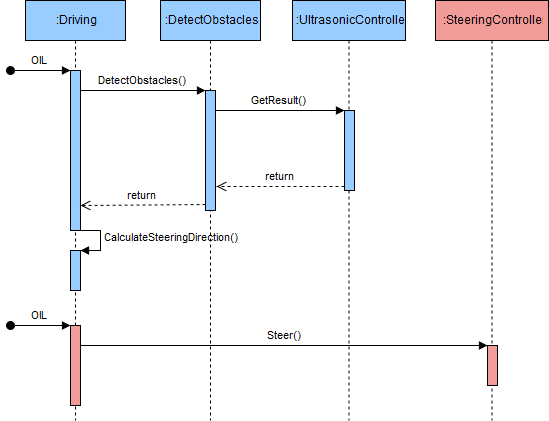
\includegraphics[width=\textwidth]{Images/Design/sequenceObstacleDetection.png}
    \caption{Sequence diagram showing the program flow while detecting obstacles and reacting to this}
    \label{fig:sequenceDetectObstacle}
\end{figure}

Task A calls the ObstacleDetection-component, which then returns results from the ultrasonic sensor. The priority of all currently saved steering-commands is then calculated and saved locally in the Driving-component. At this point the control is returned to the .oil file. 

Then task B assigns control of the CPU to the driving component a second time, which executes the highest priority steering command, which in this case is to brake the car. Task B is fully separate from obstacle detection, and regardless of which task was executed prior, task B just executes the top priority command. 

%The question is where our individual program flows are called. We have a few options, none of which seem immediately better than the rest:
%- Each component is called on its own. This makes it so the .oil programmer needs to know about the functions of all the different class functions (and where to initialize a call). This can be remedied with an interface that exposes a .Run() method. Problem here is what to do with the result of each call. If the Obstacle Detection class decides that the bus should now stop, what does it do? Does it have access to the Driving component and can it call the .Brake() function? But then all functions have access to the Driving component, which heavily increases the coupling of the program (not good). Does it expose its return value as an event that is subscribed to by the Driving component? But then the worst case execution time becomes difficult to control, because unless we know the entire program, we cannot say how many items are subscribed. Does it expose its value as a property? But then, all classes need to expose a property of the same type and also use it in the same way. Again, this increases the coupling of the program. 



\todo{Add one line descriptions of the scope (intended functionality) of the different classes. Add it into the class diagram perhaps. For instance: Maneouvre-component "high-level driving commands".Also make maneuvre inherit from Driving. Everything now goes through that instead. Driving still decides what to prioritize. Or make maneuvre a static class that can be called to get a fancy sequence of commands?}

%Driving has RequestSequenceOfCommands(list<enum DrivingCommand>, enum sender)
%drivingCommand cannot be enum, because it needs parameters, so just a class

%The solution we chose:
%One task for each component, with differing periods and deadlines.
%One task for controlling the motors.

%These tasks are all initialized from the Driving-component. So in the case where we check for obstacles, see the following sequence diagram:
%1. Oil -> Driving.DetectObstacles() -> DetectObstacles:GetResult() -> UltrasonicController.GetResult() -return to detectObstacles-> Driving.SetPriority() -return to Oil->
%2. Oil -> Driving.Steer() -> SteeringController.Steer(Command) -> MotorForSteering -return to steeringController-> MotorForSpeed

%Task 1 detects whether there are any obstacles on the track and places the suggested response (probably braking) at the top of the priority queue. 